\chapter{水声传感网络MAC协议仿真}
\section {仿真软件介绍}
\subsection{NS2}
NS2(Network Simulator,version 2)是一种面向对象的网络仿真器,本质上是一个离散事件模拟器,由UC Berkeley开发而成。它本身有一个虚拟时钟,所有的仿真都由离散事件驱动的。
NS2使用C++和Otcl作为开发语言。它包含仿真事件调度器、网络组件对象库以及网络构建模型库等。事件调度器计算仿真时间,并且激活事件队列中的当前事件,执行一些相关的事件,网络组件通过传递分组来相互通信,但这并不耗费仿真时间。所有需要花费仿真时间来处理分组的网络组件都必须要使用事件调度器。它先为这个分组发出一个事件,然后等待这个事件被调度回来之后,才能做下一步的处理工作。事件调度器的另一个用处就是计时。

\subsection{Aqua-Sim}
美国康涅狄格州大学的水下无线通迅网络研究所在NS2的基础上扩展了专门用于水下环境的仿真平台Aqua-Sim。它可以十分逼真地仿真水声信道,对信号衰减和水下包碰撞的仿真十分有效。同时它也实现了一套完整的从物理层到应用层的协议栈,各层之间可以独立发展。

 \begin{figure}[!ht]
 	\centering
 	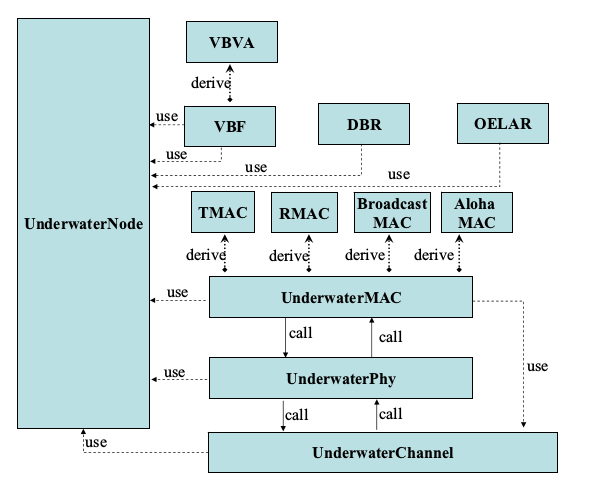
\includegraphics[scale=0.5]{figures/aq.png}
 	\caption{
 		水声传感网络
 	}
 	\label{fig:example}
 \end{figure}
\subsubsection{衰减模型}
根据传输频率$f$,距离$l$,可得吸收系数$\alpha$为
\begin{equation}
\alpha=\frac{0.11f^2}{1+f^2}+\frac{44f^2}{4100+f^2}+3.0*10^{-4}f^2+3.3*10^{-3}
\end{equation}
进而可以算出传播损失:
\begin{equation}
A(l,f)=l^k\times(10^{\frac{\alpha (f)}{10}})^l
\end{equation}
根据发送功率和传播损失可以计算出接收功率的阈值。
\begin{equation}
TxThresh=\frac{Pt}{A(l,f)}
\end{equation}

\subsubsection{能量模型}
设置IDLE,SEND,RECV三种不同的能量状态,将节点不同状态下的功率乘以状态持续时间,可以计算出节点的能耗。仿真时调用Aqua-sim的EnergyModel类,则可以进行实时的能量追踪。

\subsubsection{碰撞模型}
节点接收数据时,如果节点正处于接收状态,计算到达数据包的能量和正在接收数据包的能量之比,和比较阈值$CPThresh$进行对比。
\begin{equation}
\begin{aligned}
&if \ \ \  \frac{Pr_{\mbox{到达}}}{Pr_{\mbox{接收}}}\  > CPThresh\\
&\ \ \ \ \ \ capture(\mbox{到达数据包});\\
&else\\
&\ \ \ \ \ \ collision(\mbox{到达数据包});
\end{aligned}
\end{equation}

\section{网络性能指标}
在处理相同数据流的情况下,判断不同MAC协议下网络性能的好坏。判断网络性能时,主要统计四个网络数据指标,网络的平均时延、网络的平均吞吐量、网络的能耗、网络的数据包发送成功率。

(1)网络的平均时延是指数据包从源节点到达目的节点在网络中的传播时间。网络的时延=数据包的发送时延+数据包的传输时延+数据包的接收时延。 
\begin{equation}
\overline{T_{delay}}=\frac {\sum (T_{send}+T_{prop}T_{receive})}{\sum {N_{packet}}}
\end{equation}
(2)网络吞吐量表示网络成功发送的数据包数。网络的平均吞吐量定义为吞吐量主要用于衡量网络利用率和网络数据最大容量。
\begin{equation}
Throughout=\frac{Pkt_{recv} L_{data}}{T_{runtime}}
\end{equation}

(3)网络的数据包发送成功率是指网络中正确接收到的数据包数和总的发送数据包数的比值。
\begin{equation}
P_{succ}=\frac{Pkt_{send}}{Pkt_{recv}}
\end{equation}

(4)网络的平均能耗定义为网络中的所有节点在整个网络运行期间所消耗的总的能量与正确接收到的数据包数的比值。
\begin{equation}
\overline E=\frac{E_{consumed}}{Pkt_{recv}}
\end{equation}

\section {仿真实验一}
场景设置仿照AUV进行数据收集的情景,进行单跳移动水声网络的仿真。图中黑色代表固定节点,红色代表移动节点,红色虚线箭头指示了移动节点的移动路径。随着移动节点的移动,网络的拓扑结构会发生动态变化。固定节点会选择合适的移动节点进行数据传输。

 \begin{figure}[!ht]
 	\centering
 	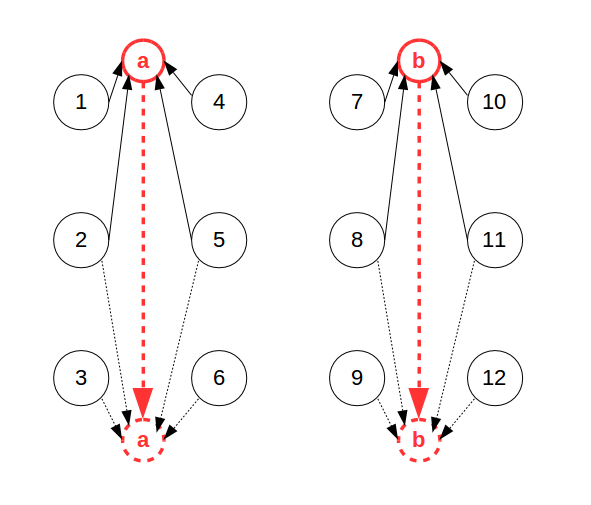
\includegraphics[scale=0.5]{figures/2scen.png}
 	\caption{
 		两移动节点场景设计
 	}
 	\label{fig:example}
 \end{figure}

节点工作参数的设置参照S2C 18/34水声通信机,参数设置如下:
\begin{table}[!htp]
	\centering
\caption{参数设置}
\begin{tabular}{m{5cm}<{\centering} m{5cm}<{\centering}}% 通过添加 | 来表示是否需要绘制竖线
	\hline  % 在表格最上方绘制横线
    参数名称& 值\\
	\hline  
	固定节点数& 12\\
	移动节点数& 2\\
	移动节点运动速度& 2.5m/s\\
	节点通信半径& 3000m\\
	相邻固定节点距离& 2000m\\
	仿真时间数& 2400s\\
	频率& 10kHz\\			
	节点传输速率& 1kbps\\
	数据包大小& 300Bytes\\
	节点发送报文功率& 30w\\				
	节点接收报文功率& 1w\\
	节点侦听报文功率& 0.2w\\
	\hline 		
\end{tabular}
\label{tab2}
\end{table}

\subsection{理论性能曲线}
按照节点的邻居节点个数和隐藏终端个数的不同,将整个仿真时间划分为不同的时间段,累计12个固定节点在所有时间段的吞吐量和,得到网络的理论吞吐量值。

仿真数据产生速率从0到0.36pkt/s(12个节点的总速率)内每0.012pkt/s的网络吞吐量,每个速率仿真十次取平均值,得到仿真吞吐量曲线。

可以看出,理论曲线与仿真曲线的走向趋势一致且误差不大,证明了理论性能曲线的准确性。
\begin{figure}[!ht]
	\centering
	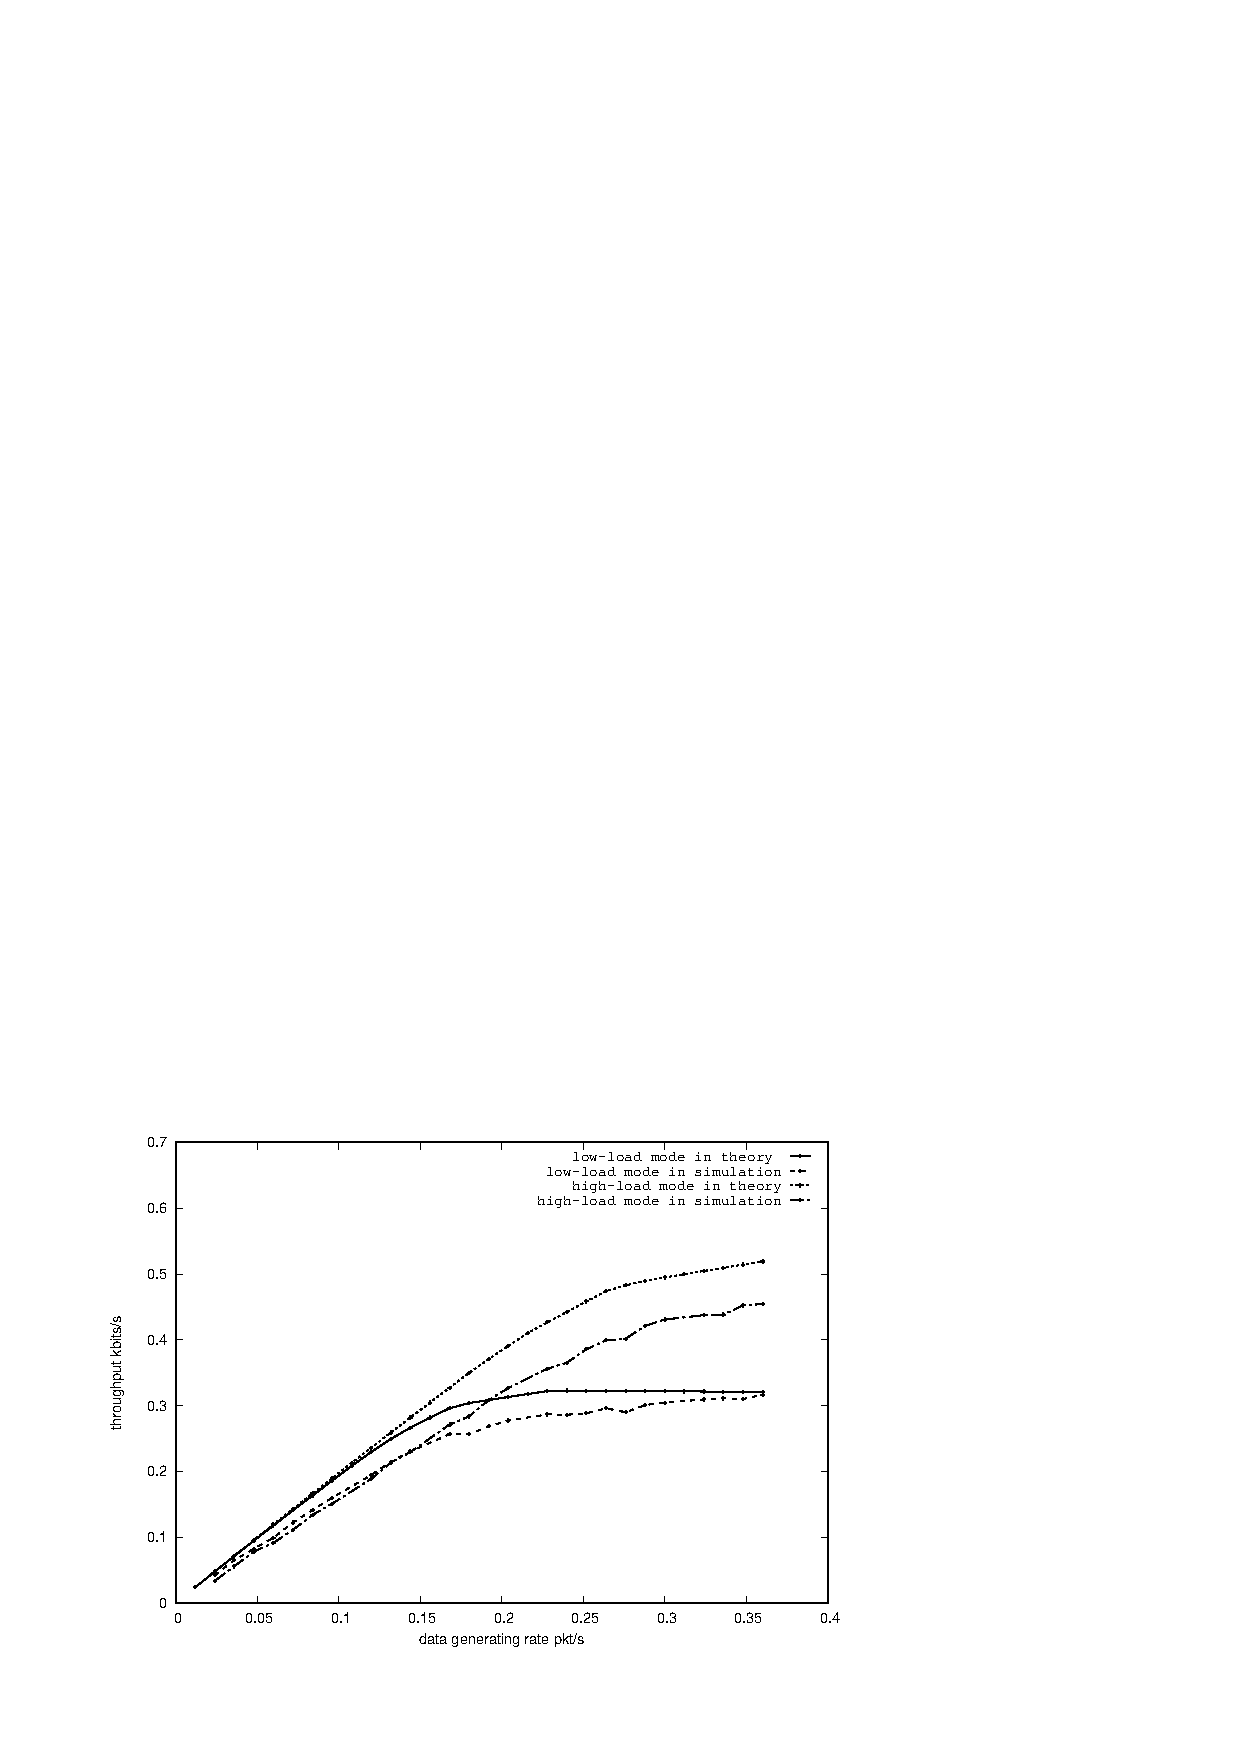
\includegraphics[scale=0.7]{figures/lilun.pdf}
	\caption{
		理论性能曲线
	}
	\label{fig:example}
\end{figure}

\subsection{结果分析}
可以看出,在网络负载较高的情况下,高负载模式协议的吞吐量远远优于低负载模式,说明握手机制在网络负载较高时引起的开销过大,影响网络性能。高负载模式的两次数据传输机制是有效的。
\begin{figure}[!ht]
	\centering
	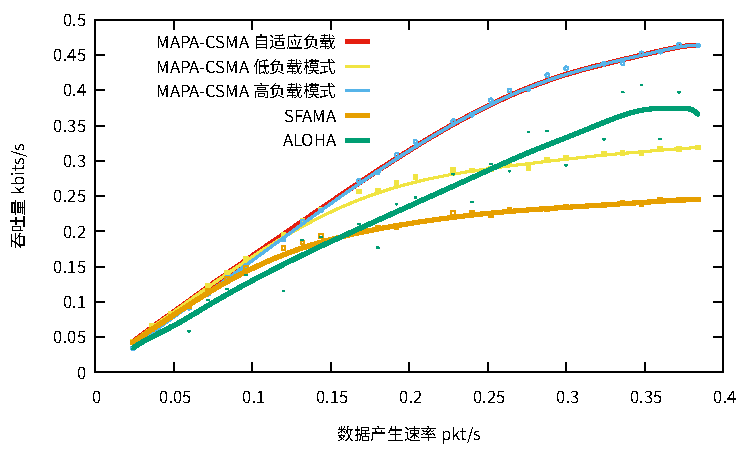
\includegraphics[scale=0.95]{figures/2nodea.pdf}
	\caption{
		吞吐量与数据产生速率关系图
	}
	\label{fig:example}
\end{figure}

由于高负载模式的两次数据传输机制需要等待第二个数据包到达才开始传输,所以在网络负载较低的情况下会引起端到端时延过大,因此自适应网络负载的数据传输机制是必要的。负载增加时,SFAMA的端到端时延会显著增加,ALOHA则对负载的变化不敏感。说明高负载网络中,握手开销极大得影响了网络性能。
\begin{figure}[!ht]
	\centering
	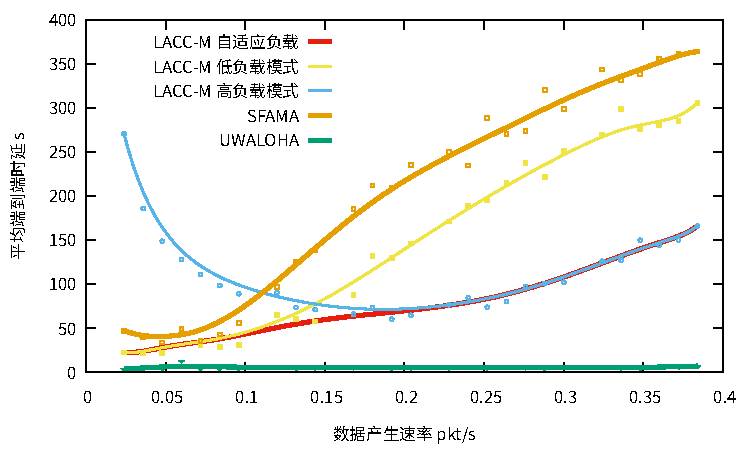
\includegraphics[scale=0.95]{figures/2nodeb.pdf}
	\caption{
		平均端到端时延与数据产生速率关系图
	}
	\label{fig:example}
\end{figure}

MAPA-MACA-CSMA协议的发送成功率显著优于SFAMA和UWALOHA协议。数据产生速率增加,即网络负载量增加对SFAMA协议的发送成功率影响较大,提出协议的改进则有效得减小了高负载下的冲突。
\begin{figure}[!ht]
	\centering
	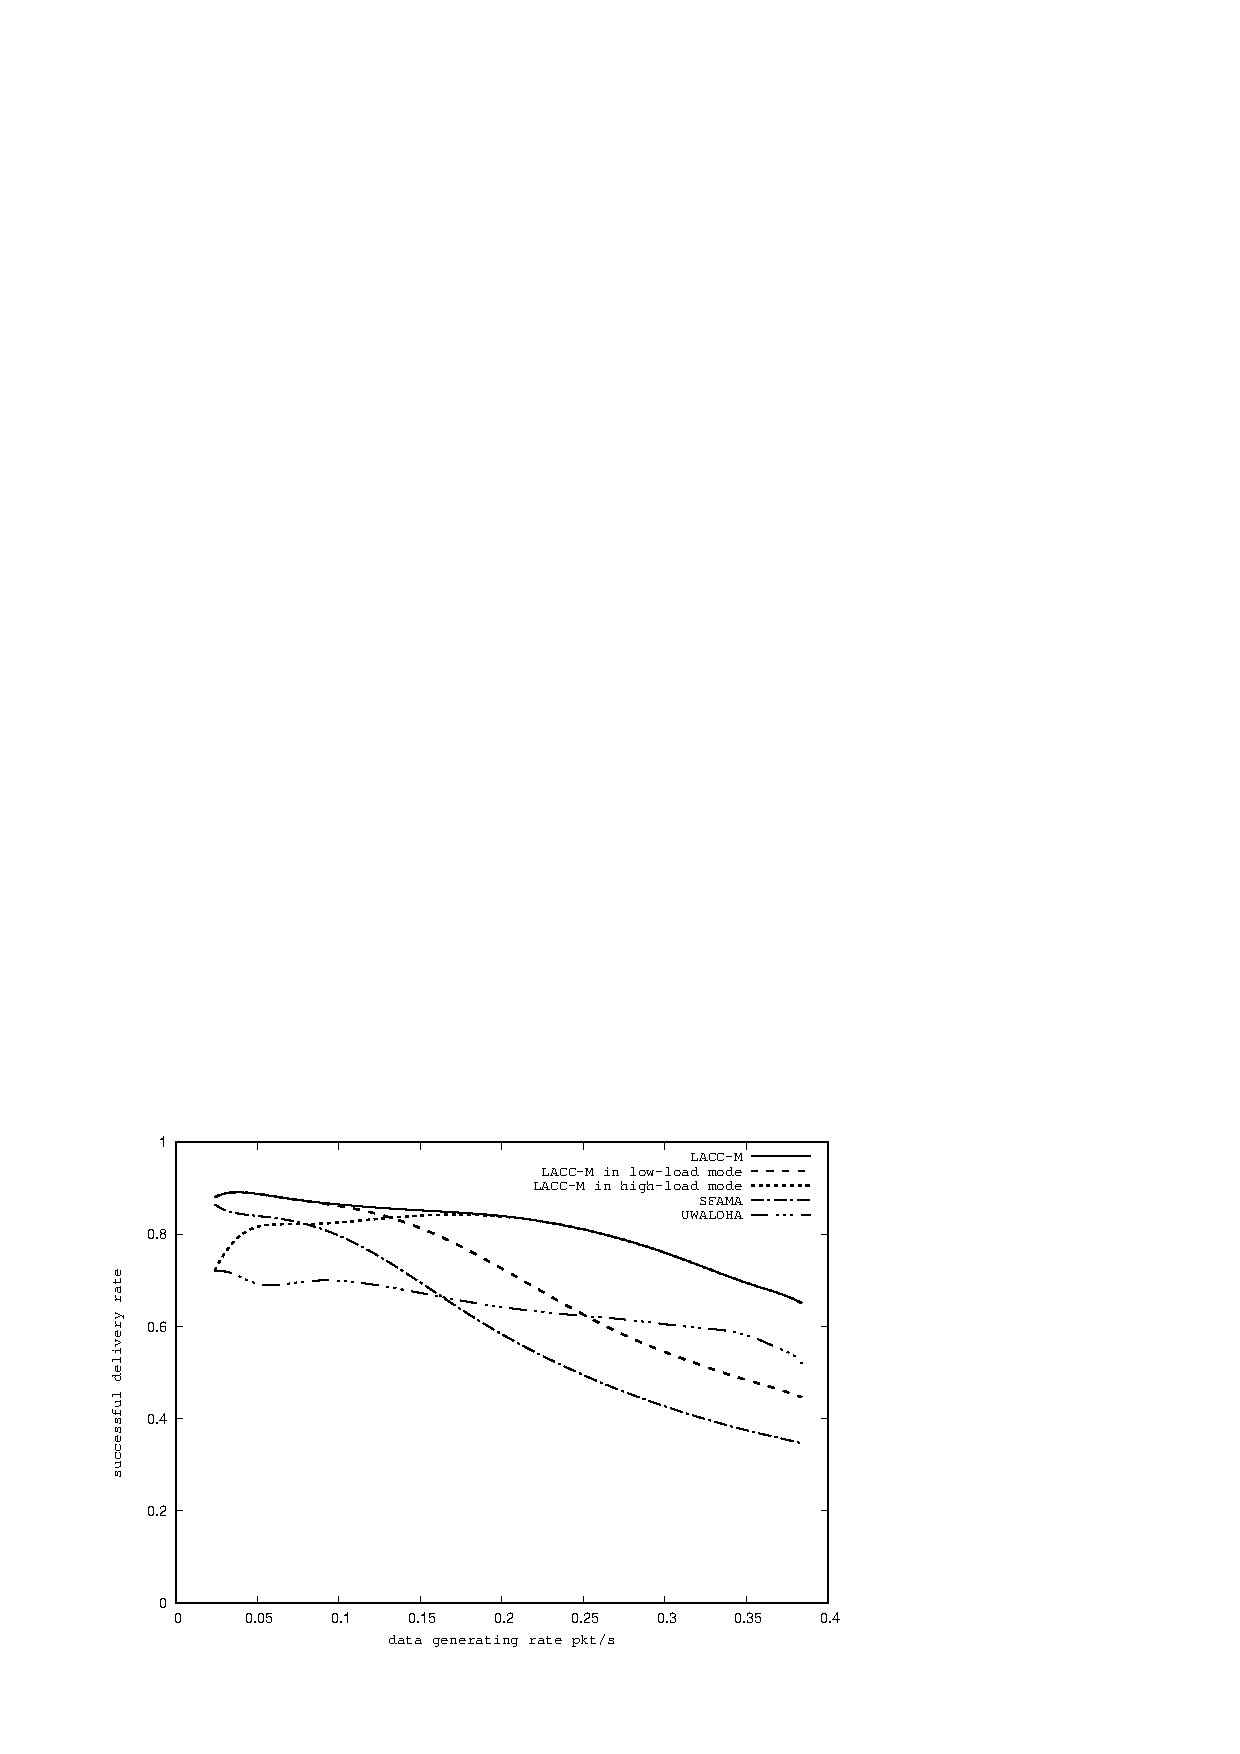
\includegraphics[scale=0.95]{figures/2nodec.pdf}
	\caption{
		发送成功率与数据产生速率关系
	}
	\label{fig:example}
\end{figure}

MAPA-MACA-CSMA协议的平均能耗在不同数据产生速率下表现都令人满意。ALOHA协议由于多次发送长数据包,所以平均能耗较高。

\begin{figure}[!ht]
	\centering
	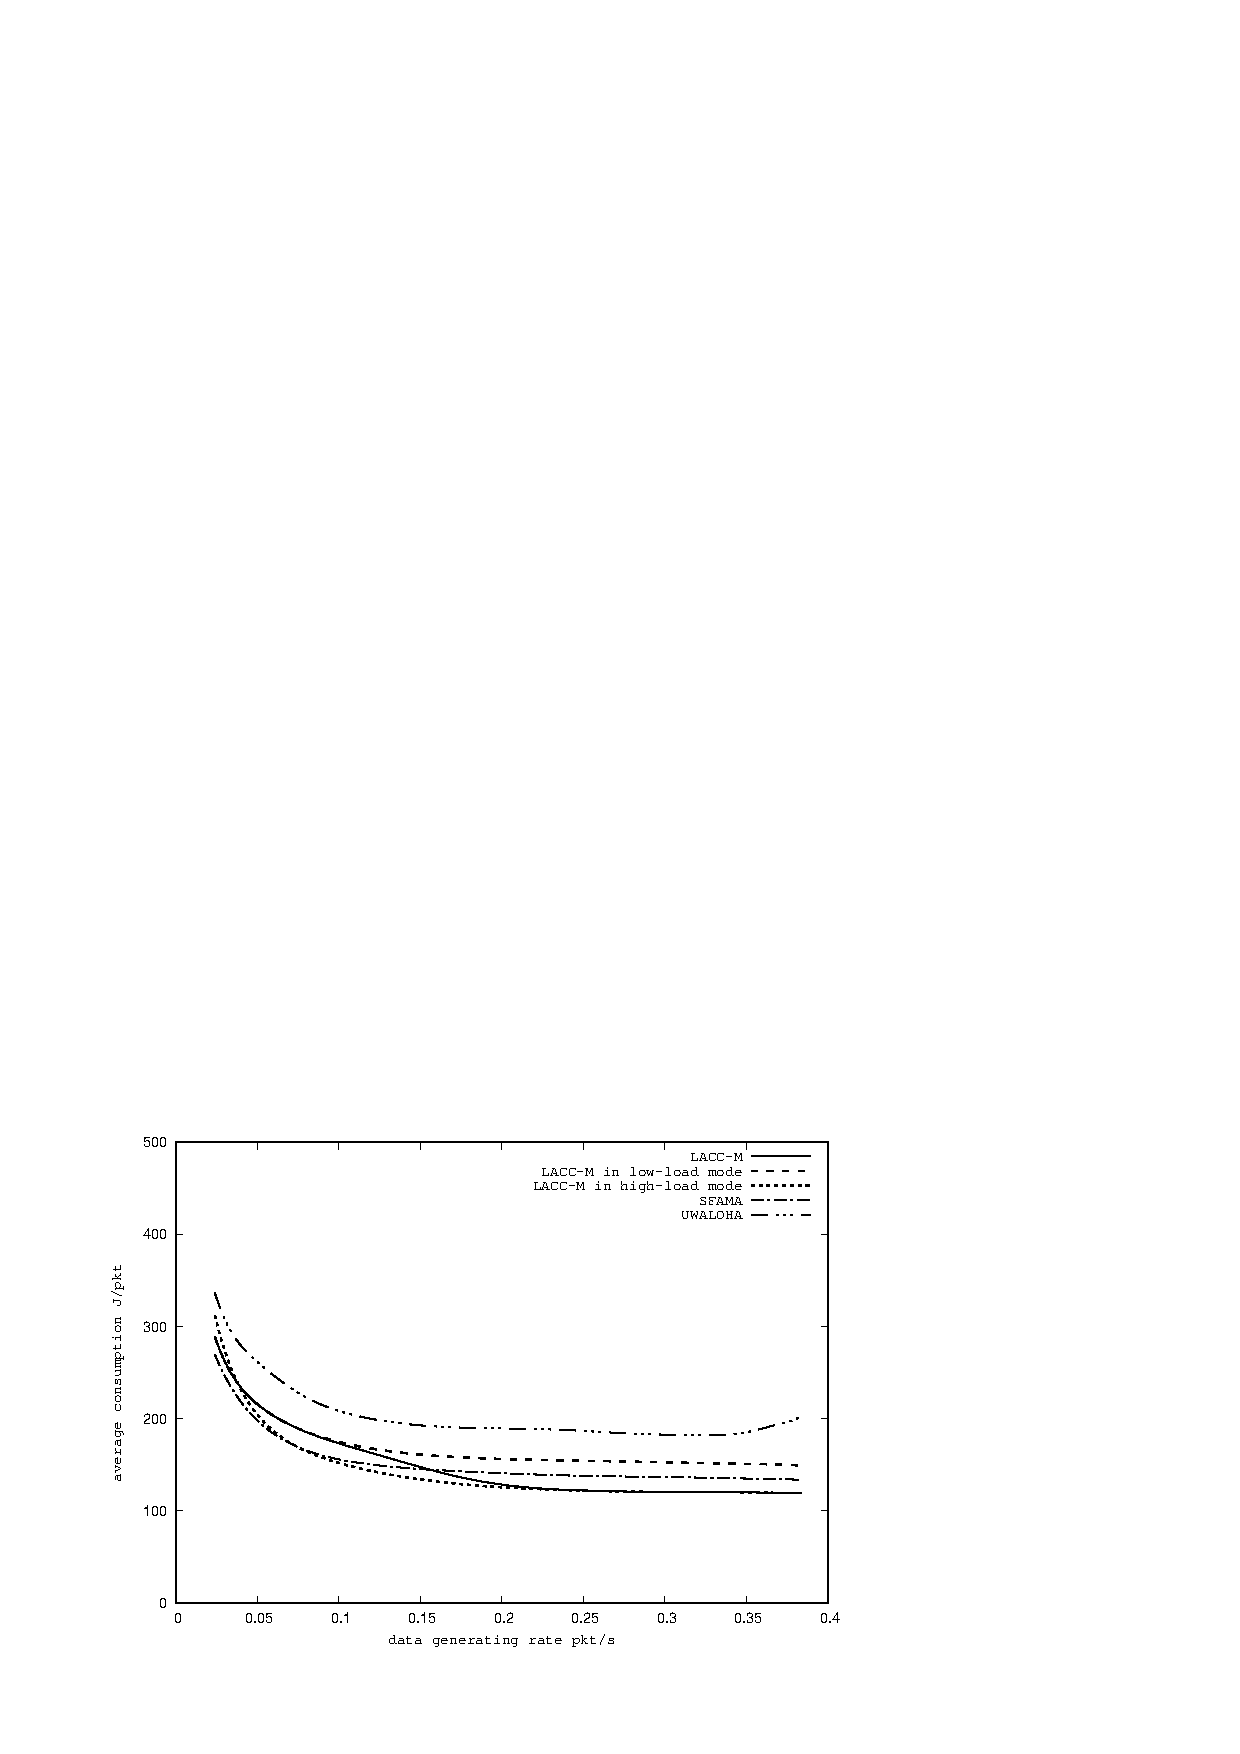
\includegraphics[scale=0.95]{figures/2noded.pdf}
	\caption{
		平均能耗与数据产生速率关系
	}
	\label{fig:example}
\end{figure}

\section {仿真实验二}
考虑到固定节点通信范围内存在多个移动节点的场景,增加移动节点数量后进行了第二组仿真。仿真参数和第一组仿真相同。移动节点的移动方向与原有的两节点方向相反,设计为由下向上,可以更好得提高信道的利用率。
\begin{figure}[!ht]
	\centering
	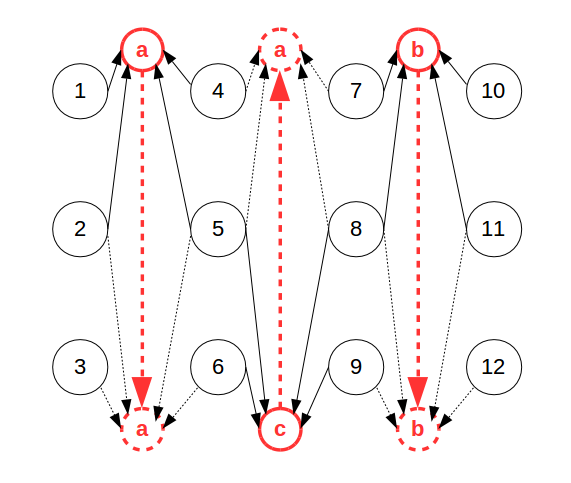
\includegraphics[scale=0.5]{figures/3scen.png}
	\caption{
		三移动节点场景设计
	}
	\label{fig:example}
\end{figure}

由于多加入了移动节点,网络拓扑的动态性变高,高负载网络的吞吐量比二移动节点的网络有所下降,网络吞吐量的临界值下降。
\begin{figure}[!ht]
	\centering
	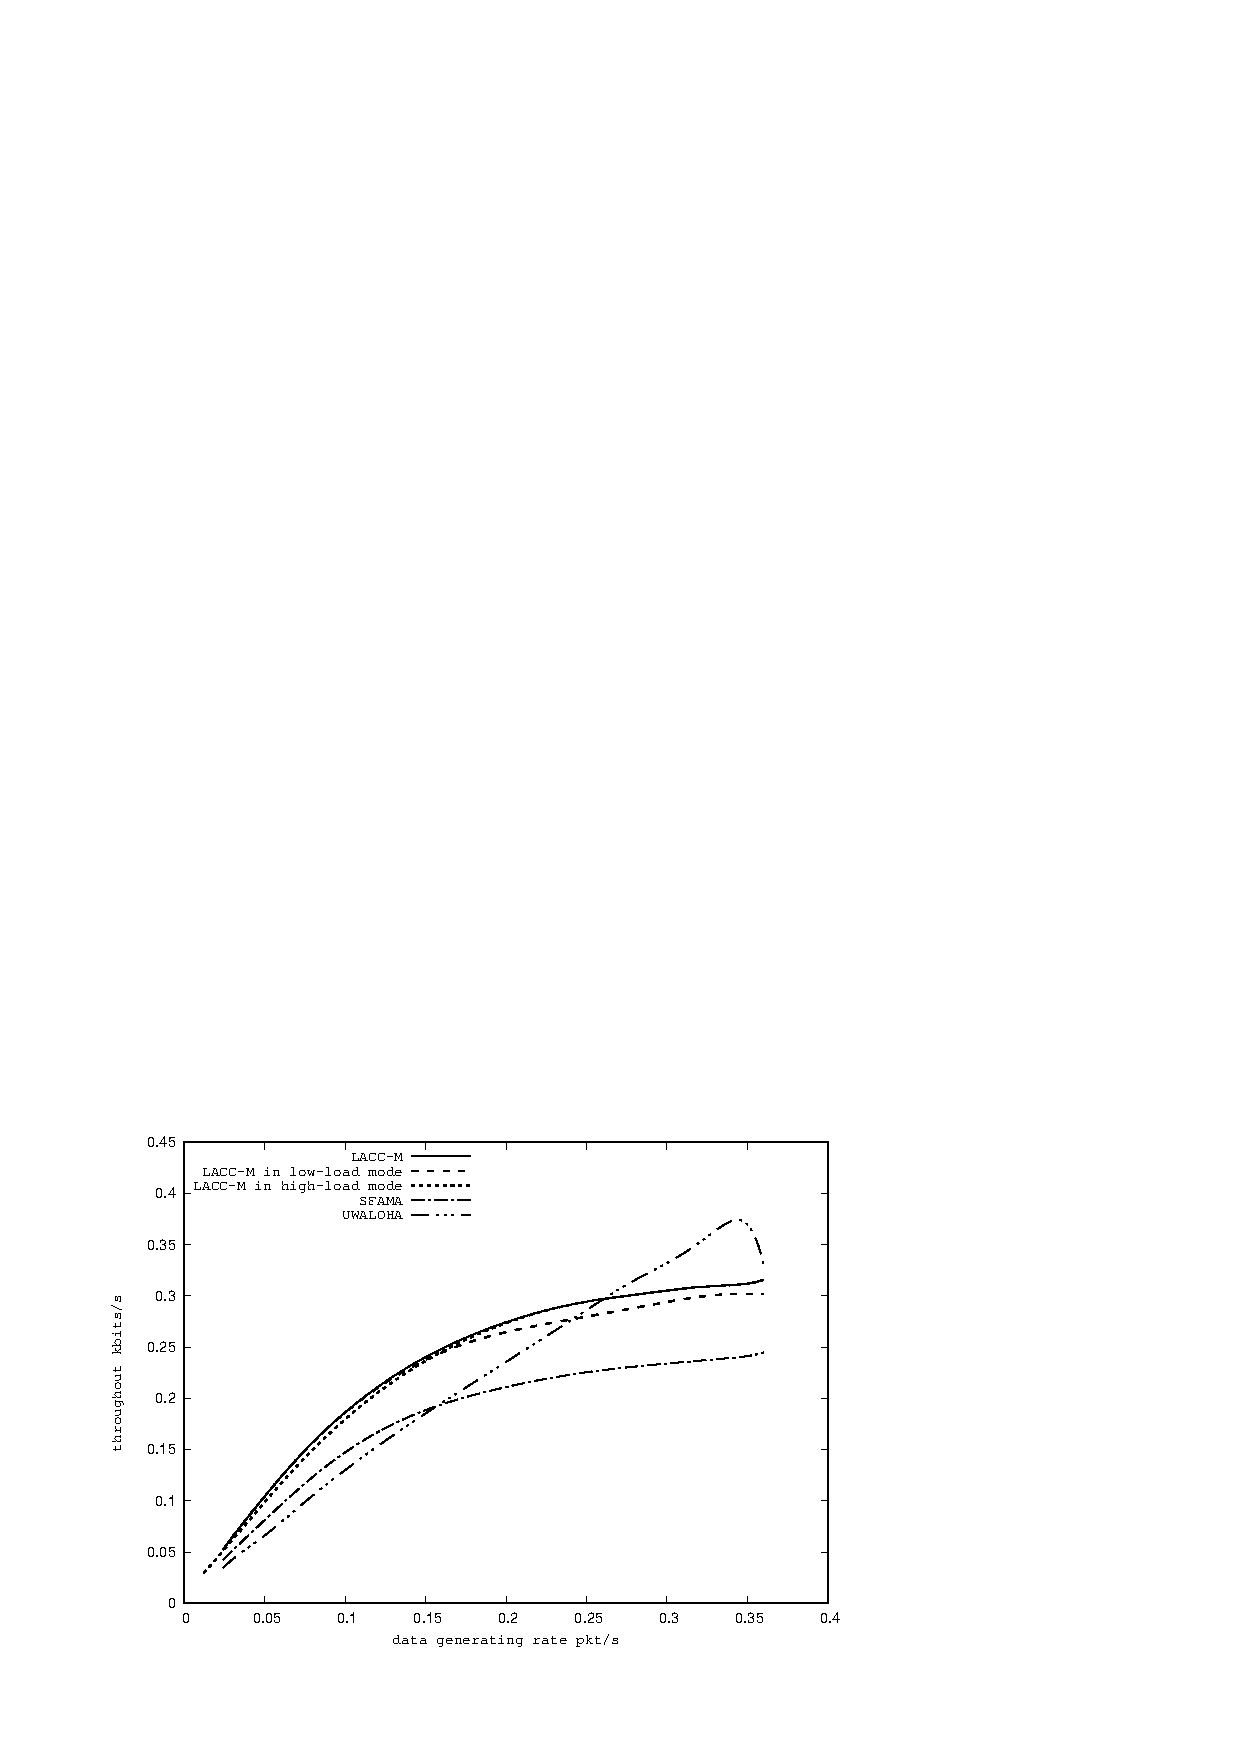
\includegraphics[scale=0.95]{figures/3nodea.pdf}
	\caption{
		吞吐量与数据产生速率关系图
	}
	\label{fig:example}
\end{figure}

可以看出在三移动节点网络中,单个移动节点承受的负载减少,所以高负载数据传输模式和低负载模式相比端到端时延优势减小,但仍然有所优化。
\begin{figure}[!ht]
	\centering
	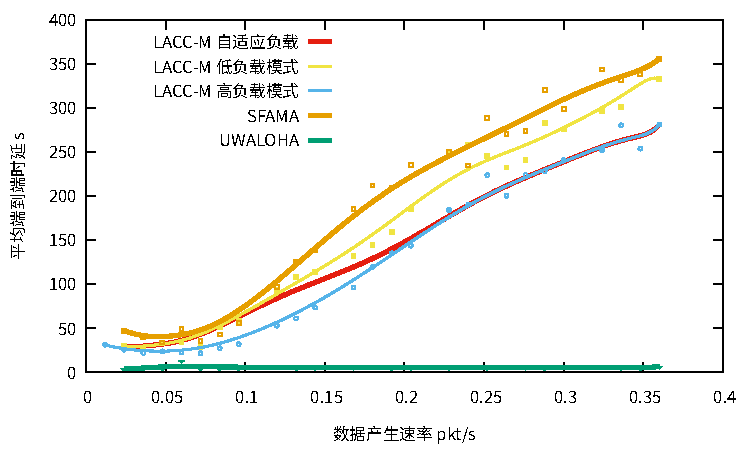
\includegraphics[scale=0.95]{figures/3nodeb.pdf}
	\caption{
		平均端到端时延与数据产生速率关系图
	}
	\label{fig:example}
\end{figure}

多加入了移动节点后,信道的利用率有所提高,所以低网络负载时的发送成功率比二移动节点模式有所提高。但是,高移动负载时,移动节点的数量增加反而会引起网络中的冲突明显增加,所以和二移动节点网络相比较,提出协议和SFAMA协议的发送成功率对网络负载的变化更敏感。
\begin{figure}[!ht]
	\centering
	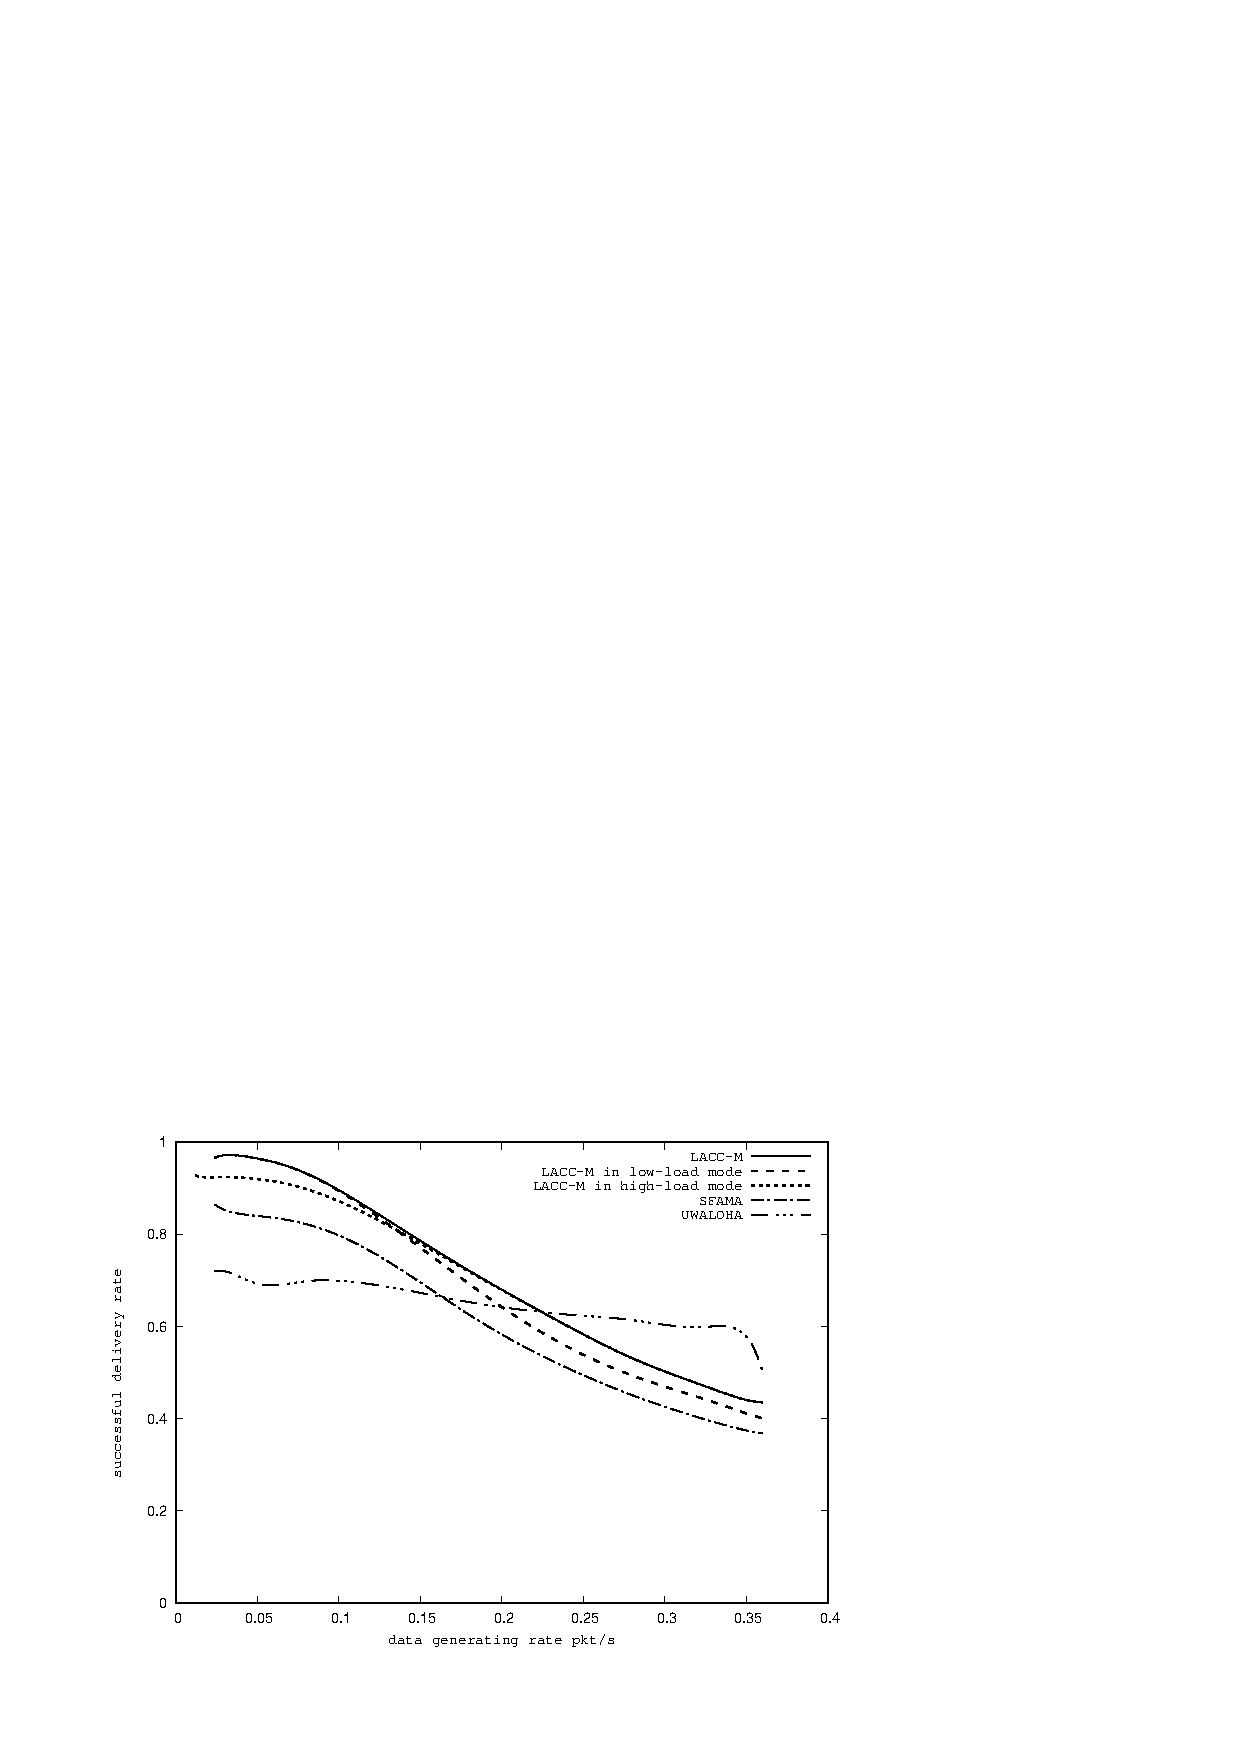
\includegraphics[scale=0.95]{figures/3nodec.pdf}
	\caption{
		发送成功率与数据产生速率关系
	}
	\label{fig:example}
\end{figure}

对于提出协议而言,多加入移动节点会带来更多的BCT包。由于仿真时固定了SFAMA和UWALOHA的节点发送结束时间并且手动设置了目标节点,没有BCT包的影响,所以提出协议的平均能耗偏高。
\begin{figure}[!ht]
	\centering
	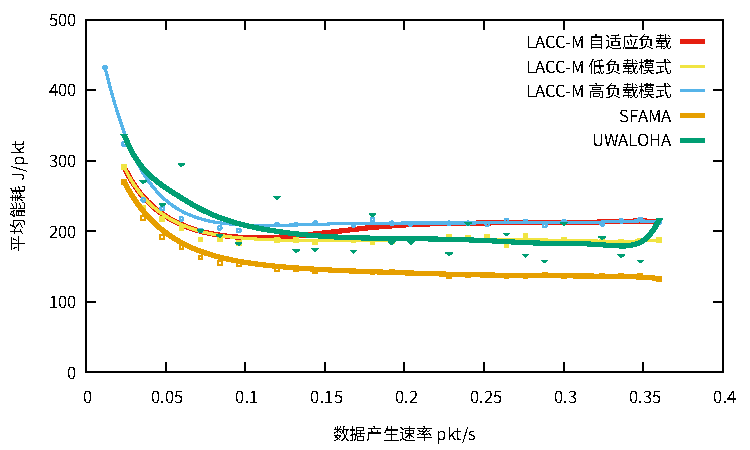
\includegraphics[scale=0.95]{figures/3noded.pdf}
	\caption{
		平均能耗与数据产生速率关系
	}
	\label{fig:example}
\end{figure}

\endinput